\section{Punti di accumulazione}

\definizione{}{
    Sia $ x_0 \in \R^{n} $, $ r>0 $, diciamo \textit{intorno (sferico)} di $ x $ di raggio $ r $
    \begin{equation}
        B_{r}(x)=\{z \in \R^{n};\, d(z,x)<r\}=\{z \in \R^{n};\, |z-x|<r\}
    \end{equation}
}

\esempio{}{
    In $ \R^{2} $, dato $ x=(x_1, x_2) $ \begin{multline*}
        B_{r}(x)=\{z=(z_1, z_2) \in \R^{2}; |z-x|<r\}=\\
        =\{z=(z_1, z_2) \in \R^{2}; (z_1-x_1)^{2}+(z_2-x_2)^{2}<r^{2}\}
    \end{multline*} 
    
    $\implies$ $ B_{r}(x) $ è un cerchio di centro $ x  $ e raggio $ r $, escluso il bordo.
}

Si indica anche con $ B(r, x) $, $ B(x,r) $, oppure $ B(x) $ se non è importante il valore del raggio.

In generale diciamo che $ I(x) $ è \textit{intorno} di $ x $ se \[
    \exists\, r>0\,\tc\, B_{r}(x) \subseteq I(x) 
\]

\definizione{}{
    Dato $ E \subseteq \R^{n} $, diciamo che $ E $ è \textit{limitato} se \[
        \exists\,R>0 \,\tc\, E \subseteq B_{R}(\underline{0}) 
    \]
}

\definizione{}{
    Sia $ E \subseteq \R^{n} $, $ x_0 \in \R^{n} $. Diciamo che $ x_0 $ è un \textit{punto di accumulazione} per $ E $ se \begin{equation}
        \forall\,r >0\, \exists\, x \in R, x \neq x_0\,\tc\, x \in B_{r}(x_0) 
    \end{equation}

    Se $ x $ di accumulazione per $ E $ $\nLeftrightarrow $ $ x \in E $
}

\esempio{}{
    Dato $ E=F\cup\{p\} $
    \begin{center}
    \begin{tikzpicture}[scale=2.5]
        \draw plot [smooth, tension=0.6] coordinates {(4.4,0.4) (5,0.2) (5.8,0.6) (6.5773,0.5421) (6.4905,1.1074)};  
        \draw [dashed] plot [smooth, tension=0.6] coordinates {(6.4905,1.1074) (5.9752,1.2828) (5.4,1.4) (4.6,1) (4.4,0.4)};
        \node at (7, 1.5) {$p$};
        \node at (5.5, 0.9) {$F$};
        \fill (6.9, 1.5) circle (0.023cm);
        \fill [green] (5,0.2) circle (0.023cm);
        \node at (5, 0.1) {\textcolor{green}{$x_0$}};
        \fill [green] (5.4,1.4) circle (0.023cm);
        \node at (5.4, 1.5) {\textcolor{green}{$x_1$}};
    \end{tikzpicture}
\end{center}
\begin{itemize}
    \item $ x_0 $ è di accumulazione;
    \item $ x_1 $ è di accumulazione;
    \item $ p $ non è di accumulazione.
\end{itemize}
}

\definizione{}{
    Se $ x_0 \in E $, $ x_0 $ non è di accumulazione, allora $ x_0 $ è un \textit{punto isolato} di $ E $.
}

\esempio{}{
    \[
        E=\big\{x=1+1/n, n \in \N\setminus \{0\}\big\}
    \]   
    $ \forall\, n $, $ x_{n}  $ non è punto di accumulazione. Se $ y \in E $ 
    
    $\implies$ $ y $ non è di accumulazione.
    
    $ a=1 $ è l'unico punto di accumulazione per $ E $, e $ 1 \notin E $. \[
        |1-x_{n}|=|1-(1+1/n)|=1/m
    \] quindi \[
        \forall\, \varepsilon>0\, \exists\, n \,\tc\, x_{n} \in B_{ \varepsilon}(1) 
    \] scegliendo $ n $ tale che $ 1/n< \varepsilon $ 
    
    $\implies$ $ n>1/ \varepsilon $
}

\esempio{}{
    $ n \in \N $ non è punto di accumulazione, $ \N $ non ammette alcun punto di accumulazione (vale anche per $ \Z $). Inoltre, un qualsiasi sottoinsieme di $ \R $, \textit{finito}, non ammette punti di accumulazione.
}

\definizione{}{Se $ E \subseteq \R^{n} $ non ammette alcun punto di accumulazione, si dice che $ E $ è \textit{discreto}

$ \N $, $ \Z $ e gli insiemi finiti sono discreti. $ \Q $ non è discreto;

numerabile $ \nRightarrow $ discreto, ma discreto $ \implies $ finito e numerabile.
}

\notazione{}{
    Dato $ E \in \R^{n} $, $ E' $ è l'insieme dei punti accumulazione di $ E $, e prende il nome di \textit{insieme derivato}.

    $ E'\neq \emptyset $ $ \iff $ $ E $ è discreto.
}

\proprieta{}{
    $ x_0 $ è di accumulazione per $ E $ 
    
    $ \iff $ $ \forall\, r > 0 $, $ B_{r}(x_0)  $ contiene infiniti punti.
    \begin{proof}
        $ \exists\, r>0 $ tale che $ \exists\, x_1\neq x_0 $, $ x_1 \in B_{r}(x_0)  $

        $ \exists\, r_1 >0 $ tale che $ x_1 \notin B_{r_{1} }(x_0)  $, $ \exists\, x_2 \in B_{r_{1} }(x_0)  $

        $ \exists\, r_2 >0 $ tale che $ x_1, x_2 \notin B_{r_{2} }(x_0)  $, $ \exists\, x_3 \in B_{r_{2} }(x_0)  $

        \dots

        Procedendo in questo modo ottengo una sequenza di punti \[
            x_1, x_2, \cdots, x_{n}, \cdots \quad \forall\, n , \, x_{n} \in B_{r}(x_0)\qedhere   
        \]
    \end{proof}
}
\proprieta{}{
    Dati due insieme $ A, B \subseteq \R $, assumiamo che $ \forall\, a \in A, b \in B $, $ a\le b $ 
    
    $\implies$ $ \sup A \le \inf B $
}

\teorema[(di Bolzano-Weierstrass)]{bolzweierstrrdsdkkslkjf}{
    Sia $ E \subseteq \R^{n} $, $ E $ limitato e $ E $ infinito. 
    
    $\implies$ $ E $ ammette almeno un punto di accumulazione $ x_0 $
}
\osservazione{
    $ E $ limitato $ \implies $ $ \exists\,r>0 $ tale che $ E \subseteq B_{r}(0)  $

    $ E $ infinito $ \iff $ $ E $ contiene infiniti punti
}
\dimostrazione{bolzweierstrrdsdkkslkjf}{
    Per semplicità dimostriamo il teorema in $ \R^{2} $\begin{itemize}
        \item [1$^{o}$ passo] Individuiamo $ x_0 $ candidato punto di accumulazione (\textit{i});
        \item [2$^{o}$ passo] dimostriamo che $ x_0 $ è davvero punto di accumulazione (\textit{ii}).
    \end{itemize} 
    \rule{7em}{.4pt}
    \begin{itemize}
        \item [(\textit{i})] Sappiamo che $ E $ è limitato 
        
        $\implies$ $ \exists\, T_{0}=[p_0, q_0]\times [r_0, s_0]  $ tale che $ E \subseteq T_{0}  $
        \begin{center}
            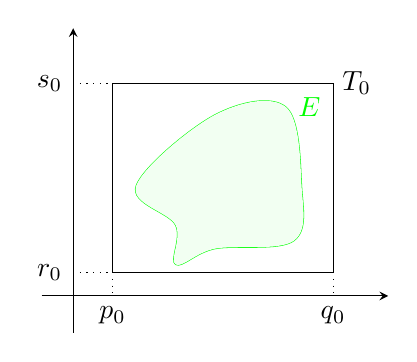
\begin{tikzpicture}
                \draw [green] plot [smooth cycle, tension=0.6] coordinates {(1, 2) (1.5, 1.5) (1.5, 1) (2, 1.2) (3, 1.3) (3.1, 2) (2.9, 3) (2, 2.9)};
                \fill [green!5] plot [smooth cycle, tension=0.6] coordinates {(1, 2) (1.5, 1.5) (1.5, 1) (2, 1.2) (3, 1.3) (3.1, 2) (2.9, 3) (2, 2.9)};
                \node at (3.2, 3) {\textcolor{green}{$E$}};  
                \draw (0.7, 0.9) -- (3.5, 0.9) -- (3.5, 3.3) -- (0.7, 3.3) -- cycle;
                \node at (3.8, 3.3) {$T_0$}; 
                \draw [-stealth] (0.2, 0.13) -- (0.2, 4); 
                \draw [-stealth] (-0.2, 0.6) -- (4.2, 0.6); 
                \draw [dotted] (0.7, 0.9) -- (0.7, 0.6);
                \draw [dotted] (3.5, 0.9) -- (3.5, 0.6);
                \draw [dotted] (0.2, 0.9) -- (0.7, 0.9);
                \draw [dotted] (0.2, 3.3) -- (0.7, 3.3);
                \node at (0.7, 0.35) {$p_0$};
                \node at (3.5, 0.35) {$q_0$};
                \node at (-0.1, 0.9) {$r_0$};
                \node at (-0.1, 3.3) {$s_0$}; 
            \end{tikzpicture}
        \end{center}

        Dividiamo $ T_{0} $ in quattro rettangoli: \[
            T_0^{1}, T_0^{2}, T_0^{3}, T_0^{4}
        \] 
        
        $\implies$ almeno uno contiene infiniti punti di $ E $. Assumiamo che sia $ T_0^{2} $

        \begin{center}
            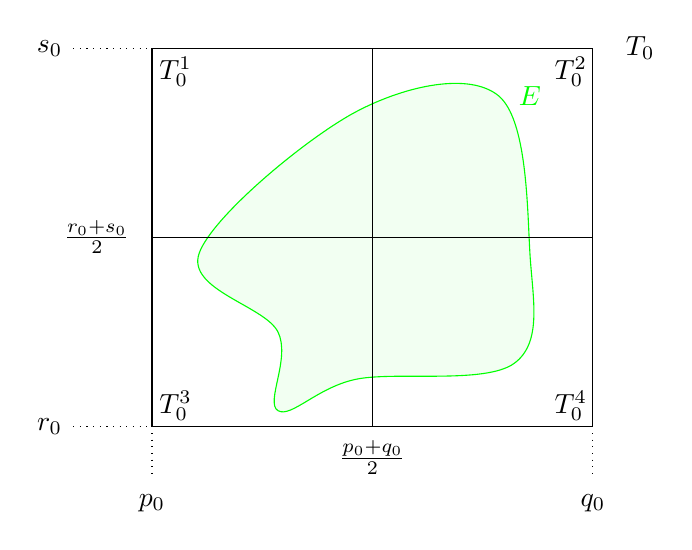
\begin{tikzpicture}[scale=2]
                \fill [green!5] plot [smooth cycle, tension=0.6] coordinates {(1, 2) (1.5, 1.5) (1.5, 1) (2, 1.2) (3, 1.3) (3.1, 2) (2.9, 3) (2, 2.9)};
                \draw [green] plot [smooth cycle, tension=0.6] coordinates {(1, 2) (1.5, 1.5) (1.5, 1) (2, 1.2) (3, 1.3) (3.1, 2) (2.9, 3) (2, 2.9)};
                \node at (3.1, 3) {\textcolor{green}{$E$}};  
                \draw (0.7, 0.9) -- (3.5, 0.9) -- (3.5, 3.3) -- (0.7, 3.3) -- cycle;
                \draw (2.1, 0.9) -- (2.1, 3.3);
                \node at (2.1, 0.7) {$\frac{p_0+q_0}{2}$};
                \node at (0.35, 2.1) {$\frac{r_0+s_0}{2}$};
                \draw (0.7, 2.1) -- (3.5, 2.1);
                \node at (3.8, 3.3) {$T_0$}; 
                \draw [dotted] (0.7, 0.9) -- (0.7, 0.6);
                \draw [dotted] (3.5, 0.9) -- (3.5, 0.6);
                \draw [dotted] (0.2, 0.9) -- (0.7, 0.9);
                \draw [dotted] (0.2, 3.3) -- (0.7, 3.3);
                \node at (0.7, 0.41) {$p_0$};
                \node at (3.5, 0.41) {$q_0$};
                \node at (0.05, 0.9) {$r_0$};
                \node at (0.05, 3.3) {$s_0$};
                \node at (0.85, 3.15) {$T_0^{1}$};
                \node at (3.36, 3.15) {$T_0^{2}$};
                \node at (0.85, 1.03) {$T_0^{3}$};
                \node at (3.36, 1.03) {$T_0^{4}$}; 
            \end{tikzpicture}
        \end{center}

        Poniamo $ T_1=T_0^{2} $, $ T_1=[p_1, q_1]\times [r_1, s_1] $\begin{align*}
            p_1& =\frac{p_0+q_0}{2}\quad &q_1=q_0\\
            r_1&=\frac{r_0+s_0}{2}\quad &s_1=s_0
        \end{align*}

        Dividiamo $ T_1 $ in quattro rettangoli. Almeno uno contiene infiniti punti di $ E $. Ne scegliamo uno: $ T_1^{3} $.

        \begin{center}
            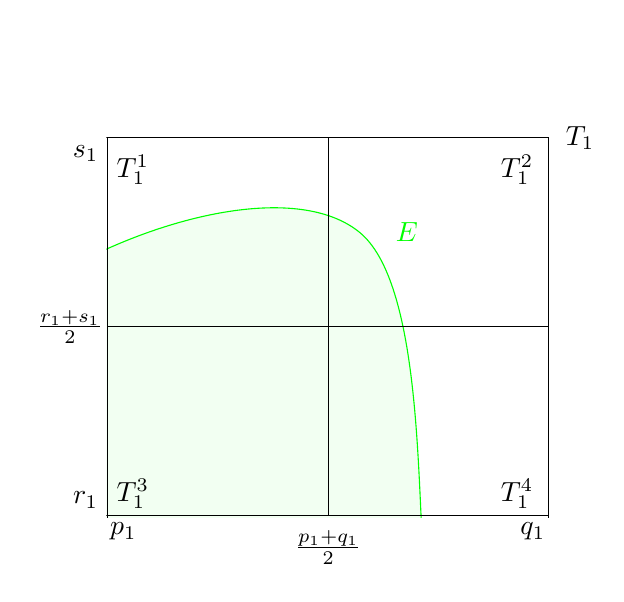
\begin{tikzpicture}[scale=4]
                \node at (2.8, 2.0) {$\frac{p_1+q_1}{2}$};
                \node at (1.98, 2.7) {$\frac{r_1+s_1}{2}$};
                \node at (2.15, 2.05) {$p_1$};
                \node at (3.45, 2.05) {$q_1$};
                \node at (2.03, 2.15) {$r_1$};
                \node at (2.03, 3.25) {$s_1$};
                \clip (2.096,2.096) rectangle (3.65,3.65);
                \fill [green!5] plot [smooth cycle, tension=0.6] coordinates {(1, 2) (1.5, 1.5) (1.5, 1) (2, 1.2) (3, 1.3) (3.1, 2) (2.9, 3) (2, 2.9)};
                \draw [green] plot [smooth cycle, tension=0.6] coordinates {(1, 2) (1.5, 1.5) (1.5, 1) (2, 1.2) (3, 1.3) (3.1, 2) (2.9, 3) (2, 2.9)};
                \node at (3.05, 3) {\textcolor{green}{$E$}};  
                \draw (0.7, 0.9) -- (3.5, 0.9) -- (3.5, 3.3) -- (0.7, 3.3) -- cycle;
                \draw (2.1, 0.9) -- (2.1, 3.3);
                \node at (2.1, 0.7) {$\frac{p_0+q_0}{2}$};
                \node at (0.35, 2.1) {$\frac{r_0+s_0}{2}$};
                \draw (0.7, 2.1) -- (3.5, 2.1);
                \node at (3.6, 3.3) {$T_1$}; 
                \draw [dotted] (0.7, 0.9) -- (0.7, 0.6);
                \draw [dotted] (3.5, 0.9) -- (3.5, 0.6);
                \draw [dotted] (0.2, 0.9) -- (0.7, 0.9);
                \draw [dotted] (0.2, 3.3) -- (0.7, 3.3);
                \node at (0.7, 0.41) {$p_0$};
                \node at (3.5, 0.41) {$q_0$};
                \node at (0.05, 0.9) {$r_0$};
                \node at (0.05, 3.3) {$s_0$};
                \node at (2.18, 3.2) {$T_1^{1}$};
                \node at (3.4, 3.2) {$T_1^{2}$};
                \node at (2.18, 2.17) {$T_1^{3}$};
                \node at (3.4, 2.17) {$T_1^{4}$};
                \draw (2.8, 2.1) -- (2.8, 3.3);
                \draw (2.1, 2.7) -- (3.5, 2.7);
            \end{tikzpicture}
        \end{center}

        Poniamo $ T_2=T_1^{3} $, $ T_2=[p_2, q_2]\times [r_2, s_2] $\begin{align*}
            p_2&=p_1\quad & q_2=\frac{p_1+q_1}{2}\\
            r_2&=r_1\quad & s_2=\frac{r_1+s_1}{2}
        \end{align*}

        Procediamo in questo modo, passo dopo passo: otteniamo una sequenza di rettangoli tutti contenenti infiniti punti di $ E $: \begin{align*}
            T_0&=[p_0, q_0]\times [r_0, s_0]\\
            T_1 \subseteq T_0 & = [p_1, q_1]\times [r_1, s_1] \\ &\implies\, s_1-r_1=\frac{s_0-r_0}{2}, \:q_1-p_1=\frac{q_0-p_0}{2}\\
            &\cdots\\
            T_{n} \subseteq T_{n-1} \subseteq \cdots \subseteq T_0 &= [p_{n} , q_{n}]\times [r_{n}, s_{n}]\\
            &\implies\, s_{n}-r_{n}=\frac{s_0-r_0}{2^{n}},\: q_{n}-p_{n}=\frac{q_0-p_0}{2^{n}}    
        \end{align*}

        Consideriamo l'insieme degli estremi destri e sinistri delle basi: \[
            P=\{p_0, p_1, \cdots, p_{n}, \cdots \},\qquad Q=\{q_0, q_1, \cdots, q_{n}, \cdots \}
        \]

        Per costruzione, $ P $ e $ Q $ sono limitati, dunque ammettono estremo superiore e inferiore. Inoltre $ \forall\, p \in P $, $ \forall\, q \in Q $, $ p<q $. Allora per la proprietà vista precdentemente, $ \sup P \le \inf Q $. Inoltre, \[
            \forall\,n,\: p_{n}\le \sup P,\: q_{n}\ge \inf Q
        \]
        quindi \[
            0\le \inf Q - \sup P \le q_{n}-p_{n}\le \frac{q_0-p_0}{2^{n}}  
        \]

        Allora $ \forall\, \varepsilon>0 $, $ 0\le \inf Q- \sup P\le \varepsilon $: è sufficiente che \[
            \frac{q_0-p_0}{2^{n}}< \varepsilon
        \] 
        
        $\implies$ $ \inf Q =\sup P $ % TODO perché posso affermare questo? non serve il teorema del confronto? posso applicarlo senza problemi? 
        \[
            x_1=\sup P = \inf Q
        \]

        Ripetiamo lo stesso ragionamento sulle altezze $ [r_{j}, s_{j}  ] $: \begin{align*}
            R&=\{r_0, r_1, \cdots, r_{n}, \cdots \}\\
            S&=\{s_0, s_1, \cdots, s_{n}, \cdots \}
        \end{align*}
        Allora $ \inf S =\sup R =x_2 $.

        Quindi $ x_0=(x_1, x_2) $ è il candidato punto di accumulazione.
        \item [(\textit{ii})] Dimostriamo che $ x_0 $ è di accumulazione:
        
        $ \forall\,n $ $ x_0 \in T_{n} $, % TODO posso dirlo senza dimostrarlo?
        ma $ T_{n} $ contiene infiniti punti di $ E $. Inoltre, $ T_{n} \subseteq T_0 $.

        $ \forall\, \varepsilon>0 $, $ \exists\, T_{c} \subseteq B_{ \varepsilon} (x_0)  $ 
        
        $\implies$ $ \forall\, \varepsilon $, $ B_{ \varepsilon}  $ contiene infiniti punti di $ E $. 
        
        $\implies$ $ x_0 $ è di accumulazione per $ E $.\qed
    \end{itemize}
}